\documentclass{article}
\usepackage{amsmath, sfmath, multicol, tkz-euclide, array, enumerate, tcolorbox, tabularray}
\renewcommand{\familydefault}{\sfdefault}
\setlength{\parindent}{0cm}
\pagestyle{empty}
\usepackage[left=1in, top=0.5in, right=1in, bottom=0.5in]{geometry}
\tikzset{>=stealth}
\tcbset{colback=white}

\newcounter{example}[section]
\newenvironment{example}[1][]{\refstepcounter{example}\par\medskip
   {\color{red}\textbf{Example~\theexample. #1}}}{\medskip}

\begin{document}

\section*{Similar Polygons}

\begin{tcolorbox}[colframe=orange!70!white, coltitle=black, title=\textbf{Today I Can}]
\begin{enumerate}
    \item Identify and apply similar polygons.
\end{enumerate}
\end{tcolorbox}
\smallskip

\begin{tcolorbox}[colframe=black!20!white, opacitybacktitle=0.1, coltitle=black, title=\textbf{Similar Figures}]
Figures that have the same shape but not the same size. The symbol for similar is $\sim$.
\end{tcolorbox}

\begin{tcolorbox}[colframe=black!20!white, opacitybacktitle=0.1, coltitle=black, title=\textbf{Similar Polygons}]
Polygons that have congruent corresponding angles and proportional lengths of corresponding sides.
\end{tcolorbox}

\begin{center}
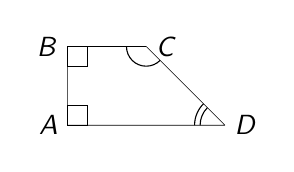
\begin{tikzpicture}
\tkzDefPoints{0/0/A, 0/1/B, 1/1/C, 2/0/D}
\tkzDrawPolygon(A,B,C,D)
\tkzLabelPoints[left](A,B)
\tkzLabelPoints[right](D,C)
\tkzMarkRightAngles[size=0.25](D,A,B A,B,C)
\tkzMarkAngle[size=0.25](B,C,D)
\tkzMarkAngle[arc=ll, size=0.35](C,D,A)
\end{tikzpicture}
\hspace{0.25in}
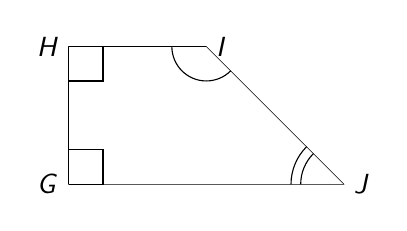
\begin{tikzpicture}[scale=1.75]
\tkzDefPoints{0/0/G, 0/1/H, 1/1/I, 2/0/J}
\tkzDrawPolygon(G,H,I,J)
\tkzLabelPoints[left](G,H)
\tkzLabelPoints[right](I,J)
\tkzMarkRightAngles[size=0.25](J,G,H G,H,I)
\tkzMarkAngle[size=0.25](H,I,J)
\tkzMarkAngle[arc=ll, size=0.35](I,J,G)
\end{tikzpicture}
\end{center}

\[
\angle A \cong \angle G, \quad \angle B \cong \angle H, \quad \angle C \cong \angle I, \quad \angle D \cong \angle J
\]

\[
\frac{AB}{GH} = \frac{BC}{HI} = \frac{CD}{IJ} = \frac{AD}{GJ}
\]

\begin{tcolorbox}[colframe=black!20!white, opacitybacktitle=0.1, coltitle=black, title=\textbf{Scale Factor}]
The ratio of corresponding side lengths of two similar figures. 
(\textit{i.e.} what you multiply or divide sides of one shape by to get the other).
\end{tcolorbox}

\begin{example}
$\triangle MNP \sim \triangle SRT$
\newline

\begin{minipage}{0.4\textwidth}
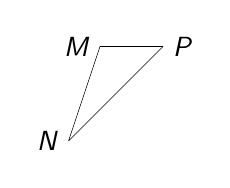
\begin{tikzpicture}[scale=0.8]
\tkzDefPoints{0/0/M, 1/0/P, -0.5/-1.5/N}
\tkzDrawPolygon(M,N,P)
\tkzLabelPoints[left](M,N)
\tkzLabelPoints[right](P)
\end{tikzpicture}
\hspace{0.25in}
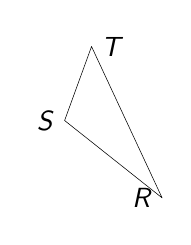
\begin{tikzpicture}[rotate=70]
\tkzDefPoints{0/0/S, 1/0/T, -0.5/-1.5/R}
\tkzDrawPolygon(S,R,T)
\tkzLabelPoints[left](S,R)
\tkzLabelPoints[right](T)
\end{tikzpicture}
\end{minipage}
\begin{minipage}{0.5\textwidth}
\begin{enumerate}[(a)]
    \item What are the pairs of congruent angles?   \vspace{0.25in}
    \item What is the extended proportion for the ratios of corresponding sides?    \vspace{0.5in}
\end{enumerate}
\end{minipage}
\end{example}

\begin{example}
Are the polygons similar? If they are, write a similarity statement and give the scale factor.
\begin{multicols}{2}
\begin{enumerate}[(a)]
    \item $JKLM$ and $TUVW$
    \item $\triangle ABC$ and $\triangle EFD$
\end{enumerate}
\end{multicols}
\begin{minipage}{0.55\textwidth}
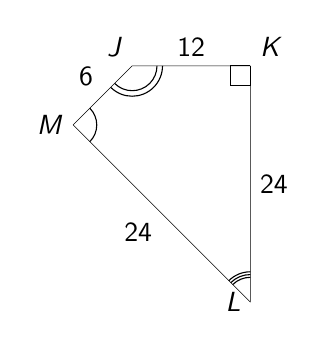
\begin{tikzpicture}
\tkzDefPoints{0/0/J, 1.5/0/K, 1.5/-3/L, -0.75/-0.75/M}
\tkzDrawPolygon(J,K,L,M)
\tkzLabelPoints[above left](J)
\tkzLabelPoints[above right](K)
\tkzLabelPoints[left](L,M)
\tkzMarkAngle[size=0.3](L,M,J)
\tkzMarkRightAngle(L,K,J)
\tkzMarkAngle[arc=ll, size=0.35](M,J,K)
\tkzMarkAngle[arc=lll, size=0.35](K,L,M)
\tkzLabelSegment[above left](J,M){6}
\tkzLabelSegment[above](J,K){12}
\tkzLabelSegment[right](K,L){24}
\tkzLabelSegment[below left](L,M){24}
\end{tikzpicture}
\hspace{0.25in}
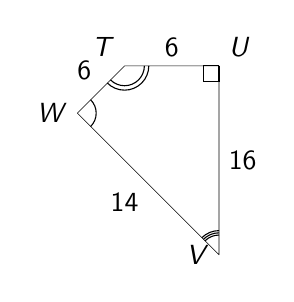
\begin{tikzpicture}[scale=0.8]
\tkzDefPoints{0/0/T, 1.5/0/U, 1.5/-3/V, -0.75/-0.75/W}
\tkzDrawPolygon(T,U,V,W)
\tkzLabelPoints[above left](T)
\tkzLabelPoints[above right](U)
\tkzLabelPoints[left](V,W)
\tkzMarkAngle[size=0.3](V,W,T)
\tkzMarkRightAngle(V,U,T)
\tkzMarkAngle[arc=ll, size=0.35](W,T,U)
\tkzMarkAngle[arc=lll, size=0.35](U,V,W)
\tkzLabelSegment[above left](W,T){6}
\tkzLabelSegment[above](T,U){6}
\tkzLabelSegment[right](U,V){16}
\tkzLabelSegment[below left](V,W){14}
\end{tikzpicture}
\end{minipage}
\begin{minipage}{0.4\textwidth}
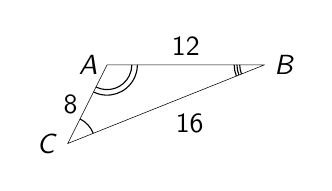
\begin{tikzpicture}
\tkzDefPoints{0/0/A, 2/0/B, -0.5/-1/C}
\tkzDrawPolygon(A,B,C)
\tkzLabelPoints[left](A,C)
\tkzLabelPoints[right](B)
\tkzLabelSegment[above](A,B){12}
\tkzLabelSegment[left](A,C){8}
\tkzLabelSegment[below right](B,C){16}
\tkzMarkAngle[size=0.35](B,C,A)
\tkzMarkAngle[arc=ll, size=0.35](C,A,B)
\tkzMarkAngle[arc=lll, size=0.35](A,B,C)
\end{tikzpicture}
\hspace{0.25in}
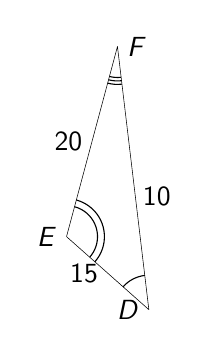
\begin{tikzpicture}[rotate=75, scale=1.25]
\tkzDefPoints{0/0/E, 2/0/F, -0.5/-1/D}
\tkzDrawPolygon(E,F,D)
\tkzLabelPoints[left](E,D)
\tkzLabelPoints[right](F)
\tkzLabelSegment[left](E,F){20}
\tkzLabelSegment[left](E,D){15}
\tkzLabelSegment[below right](F,D){10}
\tkzMarkAngle[size=0.35](F,D,E)
\tkzMarkAngle[arc=ll, size=0.35](D,E,F)
\tkzMarkAngle[arc=lll, size=0.35](E,F,D)
\end{tikzpicture}
\end{minipage}
\end{example}

\newpage 

\begin{example}
$ABCD \sim EFGD$. Find the values of the variables.
\newline\\

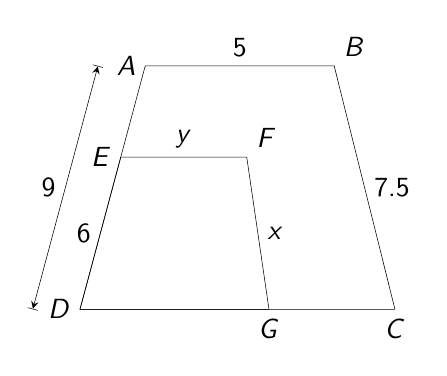
\begin{tikzpicture}[scale=0.8]
\tkzDefPoints{0/0/D, 5/0/C, 3/0/G}
\tkzDefShiftPoint[D](75:4){A}
\tkzDefShiftPoint[A](0:3){B}
\tkzDefShiftPoint[D](75:2.5){E}
\tkzDefShiftPoint[E](0:2){F}
\tkzLabelPoints[left](A,E,D)
\tkzLabelPoints[above right](B,F)
\tkzLabelPoints[below](G,C)
\tkzDrawPolygon(A,B,C,D)
\tkzDrawPolygon(E,F,G,D)
\tkzLabelSegment[left](E,D){6}
\tkzLabelSegment[above](A,B){5}
\tkzLabelSegment[above](E,F){$y$}
\tkzLabelSegment[right](F,G){$x$}
\tkzLabelSegment[right](B,C){7.5}
\tkzDefPoints{-0.75/0/H}
\tkzDefShiftPoint[H](75:4){I}
\tkzDrawSegment[|<->|, >=stealth](H,I)
\tkzLabelSegment[left](H,I){9}
\end{tikzpicture}
\end{example}

\vspace{1.25in}

\begin{tcolorbox}[colframe=black!20!white, opacitybacktitle=0.1, coltitle=black, title=\textbf{Scale Drawing}]
A drawing in which all lengths are proportional to their actual lengths.
\newline\\

The \textbf{scale} is the ratio that compares each length in the drawing to its actual length.
\[
\frac{\text{Drawing}}{\text{Actual}}
\]
\end{tcolorbox}

\bigskip 

\begin{example}
The diagram shows a scale drawing of the Golden Gate Bridge in San Francisco. The distance between the two towers is the \emph{main span}. What is the \underline{actual length} of the main span?
\vspace{0.25in}

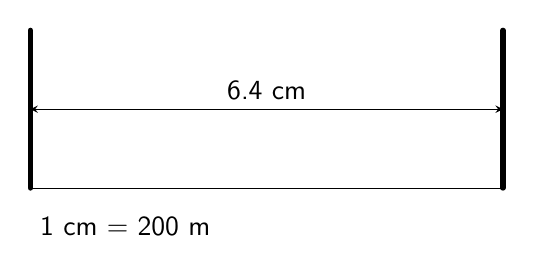
\begin{tikzpicture}
\tkzDefPoints{0/0/A, 6/0/B, 0/2/C, 6/2/D, 0/1/E, 6/1/F}
\tkzDrawSegments(A,B) 
\tkzDrawSegments[line width = 2](A,C B,D)
\tkzDrawSegment[<->, >=stealth](E,F)
\tkzLabelSegment[above](E,F){6.4 cm}
\tkzLabelPoint[below right, yshift=-0.1in](A){1 cm = 200 m}
\end{tikzpicture}
\end{example}

\end{document}
